\begin{figure}[!ht]
    \centering
    \setlength{\resLen}{4.in}
    \addtolength{\tabcolsep}{3pt}
    \begin{tabular}{cc}
        \begin{overpic}[height=\resLen]{waveoptics/pfunc/color.jpg}
			\put(2, 60){Ours}
			\put(2, 1){Single-particle}
		\end{overpic}
		&
		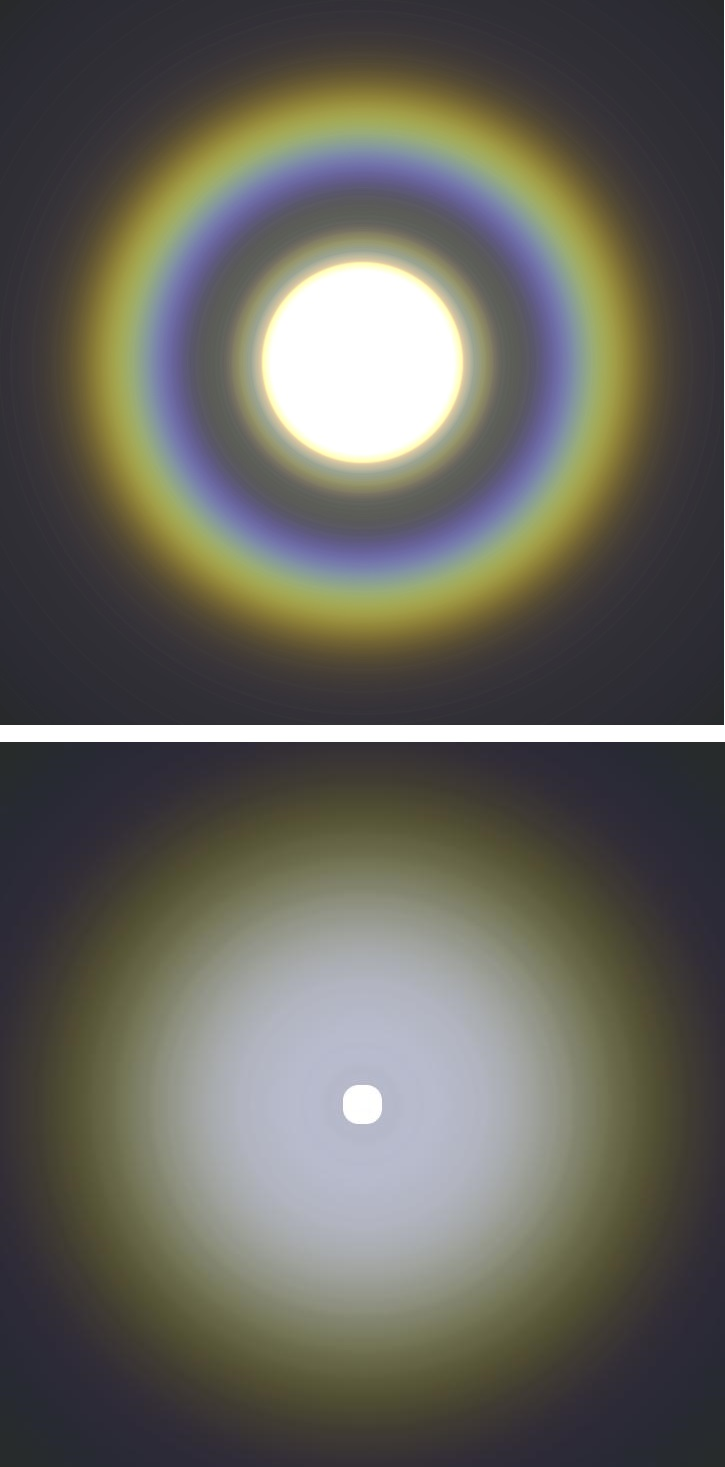
\includegraphics[height=\resLen]{waveoptics/slab/color4x_all.jpg}
        \\
        \textbf{(a)} Phase function & \textbf{(b)} Thin-slab rendering
    \end{tabular}
    \caption[Multi-spectral results]{\label{fig:waveoptics:multiwave1}
        \textbf{Multi-spectral results:} \textbf{(a)} visualizations of phase functions; \textbf{(b)} corresponding multi-spectral renderings of a thin slab lit by a small area light from behind.
        Results on the top are generated using a cluster of 100 particles with radii 500nm.
        Results on the bottom are obtained using a conventional single-particle setting.
        We used identical particle counts per differential volume for both configurations.
    }
\end{figure}
